% This is "aamas2017_sample.tex", a revised version of aamas2016_sample.tex
% This file should be compiled with "aamas2017.cls"
% This example file demonstrates the use of the 'aamas2017.cls'
% LaTeX2e document class file. It is intended for those submitting
% articles to the AAMAS-2017 conference. This file is based on
% the sig-alternate.tex example file.
% The 'sig-alternate.cls' file of ACM will produce a similar-looking,
% albeit, 'tighter' paper resulting in, invariably, fewer pages
% than the original ACM style.
%
% ----------------------------------------------------------------------------------------------------------------
% This .tex file (and associated .cls ) produces:
%       1) The Permission Statement
%       2) The Conference (location) Info information
%       3) The Copyright Line with AAMAS data
%       4) NO page numbers
%
% as against the acm_proc_article-sp.cls file which
% DOES NOT produce 1) through 3) above.
%
% Using 'aamas2017.cls' you don't have control
% from within the source .tex file, over both the CopyrightYear
% (defaulted to 20XX) and the IFAAMAS Copyright Data
% (defaulted to X-XXXXX-XX-X/XX/XX).
% These information will be overwritten by fixed AAMAS 2017  information
% in the style files - it is NOT as you are used to with ACM style files.
%
% ---------------------------------------------------------------------------------------------------------------
% This .tex source is an example which *does* use
% the .bib file (from which the .bbl file is produced).
% REMEMBER HOWEVER: After having produced the .bbl file,
% and prior to final submission, you *NEED* to 'insert'
% your .bbl file into your source .tex file so as to provide
% ONE 'self-contained' source file.
%

%
% REMEMBER: aamas2017.cls is the appropriate class for full papers and the special tracks, with the exception of the
% JAAMAS submission and industrial applications tracks. Make sure you use the appropriate class file, as follows:
% 	Extended Abstract (NOT JAAMAS): aamas2017-extabs
%	Extended Abstract for JAAMAS track: aamas2017-jaamas
%	Doctoral Consortium: aamas2017-doctoral
%	Demo: aamas2017-demo
%	Invited Presentation: aamas2017-invited
% This will ensure that the appropriate subtitle is added to your paper.
% Please ensure that you observe the page limits for your paper type.

\documentclass{aamas2017-extabs}

% if you are using PDF LaTeX and you cannot find a way for producing
% letter, the following explicit settings may help

\pdfpagewidth=8.5truein
\pdfpageheight=11truein

\begin{document}

% In the original styles from ACM, you would have needed to
% add meta-info here. This is not necessary for AAMAS 2017  as
% the complete copyright information is generated by the cls-files.


\title{Optimizing Resource Allocation with Intelligent Agents}

% AUTHORS

% You need the command \numberofauthors to handle the 'placement
% and alignment' of the authors beneath the title.
%
% For aesthetic reasons, we recommend 'three authors at a time'
% i.e. three 'name/affiliation blocks' be placed beneath the title.
%
% NOTE: You are NOT restricted in how many 'rows' of
% "name/affiliations" may appear. We just ask that you restrict
% the number of 'columns' to three.
%
% Because of the available 'opening page real-estate'
% we ask you to refrain from putting more than six authors
% (two rows with three columns) beneath the article title.
% More than six makes the first-page appear very cluttered indeed.
%
% Use the \alignauthor commands to handle the names
% and affiliations for an 'aesthetic maximum' of six authors.
% Add names, affiliations, addresses for
% the seventh etc. author(s) as the argument for the
% \additionalauthors command.
% These 'additional authors' will be output/set for you
% without further effort on your part as the last section in
% the body of your article BEFORE References or any Appendices.

%\numberofauthors{9} %  in this sample file, there are a *total*
% of NINE authors. SIX appear on the 'first-page' (for formatting
% reasons) and the remaining three appear in the \additionalauthors section.
%

\numberofauthors{3}

\author{
% You can go ahead and credit any number of authors here,
% e.g. one 'row of three' or two rows (consisting of one row of three
% and a second row of one, two or three).
%
% The command \alignauthor (no curly braces needed) should
% precede each author name, affiliation/snail-mail address and
% e-mail address. Additionally, tag each line of
% affiliation/address with \affaddr, and tag the
% e-mail address with \email.
% 1st. author
\alignauthor
Lucas O. Souza\\
       \affaddr{University of Brasilia}\\
       \affaddr{PO Box 4466}\\
       \affaddr{Brasilia, Brazil}\\
       \email{lucasosouza@gmail.com}
% 2nd. author
\alignauthor
Celia G. Ralha\\
       \affaddr{University of Brasilia}\\
       \affaddr{PO Box 4466}\\
       \affaddr{Brasilia, Brazil}\\
       \email{ghedini@unb.br}
% 3rd. author
\alignauthor
Bruno W. P. Hoelz\\
       \affaddr{University of Brasilia}\\
       \affaddr{PO Box 4466}\\
       \affaddr{Brasilia, Brazil}\\
       \email{bhoelz@unb.br}
}
% END \author command

%% There's nothing stopping you putting the seventh, eighth, etc.
%% author on the opening page (as the 'third row') but we ask,
%% for aesthetic reasons that you place these 'additional authors'
%% in the \additional authors block, viz.
%\additionalauthors{Additional authors: John Smith (The Th{\o}rv{\"a}ld Group,
%email: {\texttt{jsmith@affiliation.org}}) and Julius P.~Kumquat
%(The Kumquat Consortium, email: {\texttt{jpkumquat@consortium.net}}).}
%\date{30 July 1999}
%% Just remember to make sure that the TOTAL number of authors
%% is the number that will appear on the first page PLUS the
%% number that will appear in the \additionalauthors section.

\maketitle

\begin{abstract}
Playing the stock market is one of the many frontiers of applied artificial intelligence. The problem of optimizing asset allocation within a portfolio to yield a return above the market is a hard problem. Current approaches include multi-agent systems in which the task of gathering data, predicting trend and choosing assets are divided between specialized cooperative agents that simulate the environment of an investment fund. This paper builds upon existing models to create ORACLIA (\textbf{O}ptimizing \textbf{R}esource \textbf{A}llocation and \textbf{C}apital \textbf{L}ucrativeness with \textbf{I}ntelligent \textbf{A}gents), a multi-agent system for portfolio optimization in the Brazilian Stock Market (Bovespa). A multi-agent architecture was defined and implemented with the use of machine learning classification models to generate buy and sell signals based on the success or failure probability of a predefined strategy. The classification models are able to predict success or failure of a strategy with over 80\% accuracy for certain assets. These models successfully replaces the traditional approach that uses regression to predict stock price trends. Backtesting results, conducted in a simulated environment with actual stock market data from 2015 and 2016, show ORACLIA achieves net results up to eight times higher than single asset portfolios or general benchmarks such as Ibovespa, the main index for Bovespa.
\end{abstract}

\keywords{multi-agent systems; intelligent agents; supervised learning; asset allocation; stock market; stock price prediction}

\section{Introduction}
\label{sec-intro}
Choosing to buy assets based on a predictive upward trend is a discipline that dates back to the early days of capitalism. The introduction of artificial intelligence (AI) methods in investment portfolio management and the rise of machine learning have drawn a lot of attention to the field, which promises big rewards for those who can crack the challenge. 

When a bank or a hedge fund decides which stock to buy and which to sell, many players are involved in the decision. There are those who gather the data, those who process it and try to come up with stock price trends, and those who use this information to trade. The described players' rules can be well represented by multi-agent systems that resemble real day-to-day environments.

Considering the above scenario, this paper presents ORACLIA, a multi-agent system for portfolio optimization in the Brazilian Stock Market (Bovespa). It was built upon existing approaches in which the task of gathering data, predicting trend and choosing assets are divided among specialized, cooperative agents that simulate an investment fund. Each agent in ORACLIA reflects the role that would be occupied by an employee in a hedge fund structure. The behavior of each agent is heavily based on AI methods, such as supervised learning and reinforcement learning, to add intelligence to the designed system.

\section{Related Work}
\label{sec-review}

In \cite{hafezi2015bat} we find a multi-agent systems for stock price prediction, in a four-layered architecture. Similar approaches are found in previous works \cite{lee2007multiagent,luo2002multi, rahimi2009multi}. While \cite{lee2007multiagent} is focused on predicting stock prices trend, \cite{luo2002multi} is concerned with investment decisions that optimize asset allocation. The work of  \cite{de2013automated} presents a multi-agent system, composed of coaches and advisors, that cooperate to optimize a portfolio based on the analysis of assets risk.

Significant work have also been done in the field of agents operating in a simulated stock market environment \cite{Sherstov2005, PXS, Bloembergen2015}.

There is a vast literature on the topic of using non-linear regressors to predict stock prices. There seems to be a focus on neural networks, regarded as the state of the art in non-linear regressors in \cite{nemes2013data,hafezi2015bat,chenoweth1996embedding}. The designed systems have been applied to a variety of markets, from Romania \cite{nemes2013data} to Germany \cite{hafezi2015bat} and Brazil \cite{jabbur2014design}. 

\section{ORACLIA Model}
\label{sec-model}

The starting point of defining a multi-agent architecture is setting its goals. The main goal of the system in this case is to maximize the return of the portfolio, and one of the relevant sub-goals is to increase precision in predicting whether or not a predefined strategy will be successful. 
ORACLIA's architecture is depicted in Figure~\ref{fig-architecture}. 

The Fund Manager agent receives input from the user of which assets to consider, how much capital to allocate and a time frame, and outputs buy and sell recommendations. In order to obtain the recommendations, the manager requests investment strategies from the Strategy Agents. Each strategy agent has access to distinct Data Provider agents that collect relevant data available online, store and provide it when requested. 

Strategy Agents also have access to a back-testing service that is used to test its strategies against historic data. Strategy agents respond to the Fund Manager with their best strategies considering the constraints provided by the user. Finally, the Fund Manager can provide one or more of strategies for the user to choose from.

\begin{figure}[htb]
\centering
  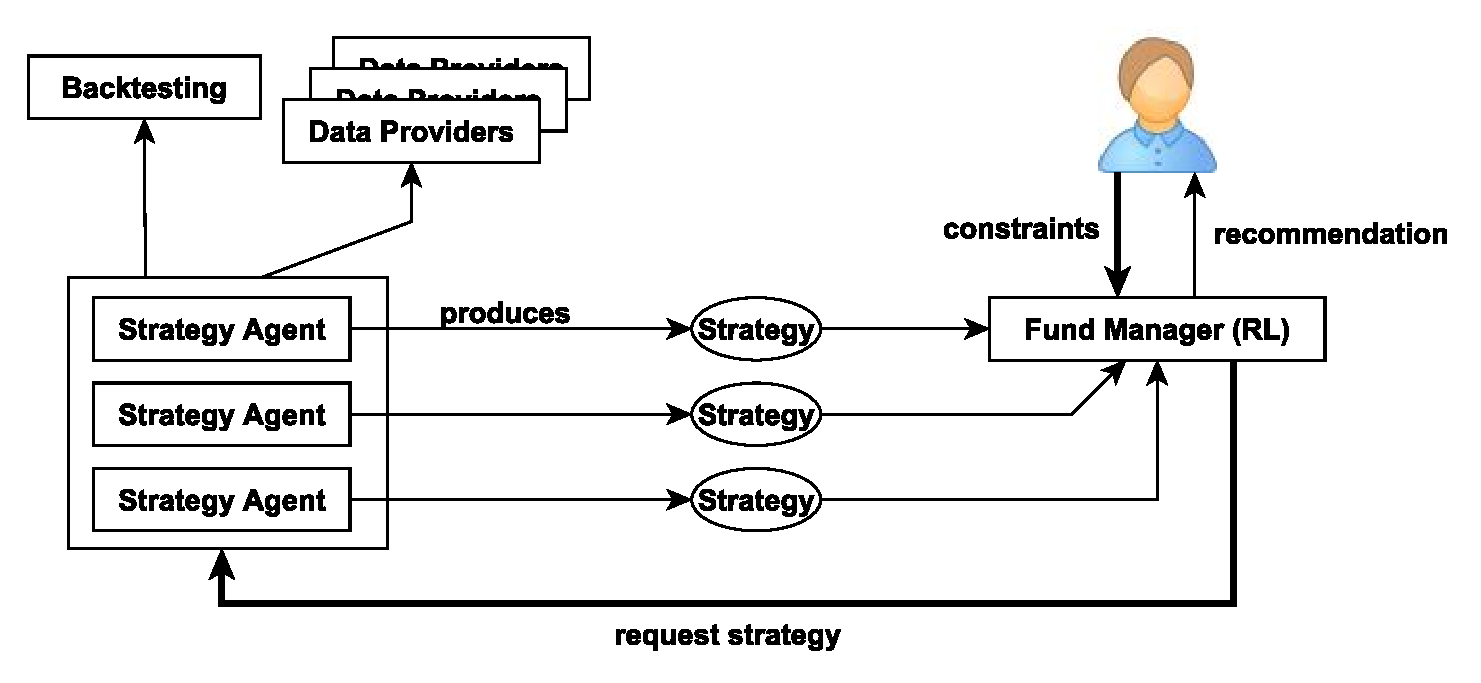
\includegraphics[scale=0.32]{modelo-lucas.eps}\\
  \caption{Architecture of the ORACLIA multi-agent system}
  \label{fig-architecture}
\end{figure}

\subsection{Stock Price Prediction as a Classification Problem}
\label{sec-proposed}

The usual approach when dealing with stock price trend prediction is using non-linear regression models to predict future stock prices. Regression is a complex problem, with unsatisfactory results when dealing with stock prices. Predicting the price three days ahead (or three minutes ahead with intraday stock price) is a much harder problem than predicting one day ahead.

To avoid this pitfall, ORACLIA turns predicting stock price trend into a classification problem, contrary to the common approach of using non-linear regressors. The approach is based on a predefined strategy, which the agent holds as fixed. The strategy will tell which type of asset to buy, when, and when to short the position.

The simplest strategy, called swing trade, is buying an asset, and selling it if the price increases or decreases X\% within the next N days. Parameters X and N can be optimized.

With a strategy defined, the strategy agent evaluates the entire training set, and for each observation creates a binary label, which indicates whether the strategy would have worked or not if applied on that day. The success/failure label will be the label learned by the classifier.

The goal of the classification problem is, given the variables for the current day, to define whether applying a strategy will be successful or not. There is an inherent trade-off as we are disregarding additional information that would be obtained in the regression-based approach, such as the expected price of the asset, to obtain a simpler model which can be trained to higher precision.

\section{Implementation}
\label{sec-implementation}

ORACLIA was implemented using several open source Python packages. Scikit Learn \cite{scikit-learn} was used for machine learning algorithms and data preprocessing features. Pandas \cite{mckinney2010data} and matplotlib \cite{hunter2007matplotlib}, Seaborn \cite{michael_waskom_2014_12710} and Jupyter notebooks \cite{perez2007ipython} were used for data wrangling and visualization. The agents implementation was done in the \emph{Smart Python Agents Development Environment} (SPADE) \cite{jabbur2014design}, which is a FIPA-compliant multi-agent environment based on JADE. The infrastructure used was a Mac 2014 notebook, with 8 cores and 16 GB of RAM. Future implementations will be based on Amazon Elastic Search for better scalability.

\subsection{Experiments}
\label{sec-expe}

A prototype of ORACLIA was tested with the Brazilian stock market (Bovespa). Data from the five stocks with higher weight in the Ibovespa index were used in the experiments: ABEV3, BBDC4, ITUB4, PETR4, and VALE5. The training data considered the period from 2012 to 2014, while the evaluation data considered the period from Jan. 2015 to Oct. 2016. 

For each stock, a strategy agent was implemented, using a swing trade strategy and a kNN classifier. In backtesting, the strategy agents achieved precision as high as 80\% in predicting whether or not a strategy would be successful. The fund manager agent simulated an investment portfolio in the period of 2015-2016. The return of investment achieved in the period is eight times higher than the IBOVESPA index gains or any of the traded stocks treated separately, as shown in Figure~\ref{fig-performance}. 

\begin{figure}[htb]
\centering
  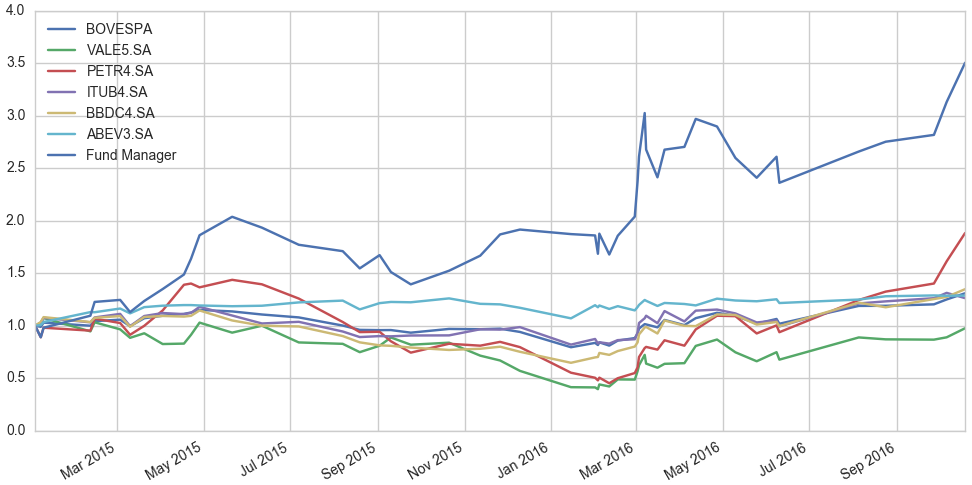
\includegraphics[scale=0.34]{performance-article2.png}
  \caption{Performance from Jan. 2015 to Oct. 2016, total portfolio valuation of 252\% compared to 32\% valuation of IBOVESPA index in the same period}
  \label{fig-performance}
\end{figure}

\section{Conclusions}
\label{conclu}

This paper presented ORACLIA, a multi-agent system to solve the optimal asset allocation problem, aiming to maximize return of an investment portfolio. To do so, several AI methods are employed, including a novel approach to predict stock price trends using non-parametric classifiers.

The multi-agent approach of ORACLIA, where autonomous agents can operate independently in different locations, facilitates distribution and scalability. The use of the FIPA-ACL communication protocol simplifies the introduction of agents from other FIPA-compliant platforms.

Since the agents in ORACLIA's architecture reflect roles in an investment fund structure, the proposed approach could be deployed as part of the organization. Likewise, human agents could also play the role of a Strategy Agent or even the Fund Manager in the system.

The preliminary results found in the implementation of ORACLIA are promising, and can be further improved by increasing the number of assets per portfolio and the range of strategies applied for each asset.

% produce the bibliography for the citations in your paper.
% \bibliographystyle{abbrv}
% \bibliography{references} 

\begin{thebibliography}{10}

\bibitem{Bloembergen2015}
D.~Bloembergen, D.~Hennes, S.~Parsons, and K.~Tuyls.
\newblock Survival of the chartist: An evolutionary agent-based analysis of
  stock market trading.
\newblock In {\em Proceedings of the 2015 International Conference on
  Autonomous Agents and Multiagent Systems}, AAMAS '15, pages 1699--1700,
  Richland, SC, 2015. International Foundation for Autonomous Agents and
  Multiagent Systems.

\bibitem{chenoweth1996embedding}
T.~Chenoweth, Z.~Obradovic, and S.~S. Lee.
\newblock Embedding technical analysis into neural network based trading
  systems.
\newblock {\em Applied Artificial Intelligence}, 10(6):523--542, 1996.

\bibitem{de2013automated}
P.~A.~L. de~Castro and J.~S. Sichman.
\newblock Automated asset management based on partially cooperative agents for
  a world of risks.
\newblock {\em Applied Intelligence}, 38(2):210--225, 2013.

\bibitem{hafezi2015bat}
R.~Hafezi, J.~Shahrabi, and E.~Hadavandi.
\newblock A bat-neural network multi-agent system (bnnmas) for stock price
  prediction: Case study of dax stock price.
\newblock {\em Applied Soft Computing}, 29:196--210, 2015.

\bibitem{hunter2007matplotlib}
J.~D. Hunter.
\newblock Matplotlib: A 2d graphics environment.
\newblock {\em Computing In Science \& Engineering}, 9(3):90--95, 2007.

\bibitem{jabbur2014design}
E.~Jabbur, E.~Silva, D.~Castilho, A.~Pereira, and H.~Brand{\~a}o.
\newblock Design and evaluation of automatic agents for stock market intraday
  trading.
\newblock In {\em Proceedings of the 2014 IEEE/WIC/ACM International Joint
  Conferences on Web Intelligence (WI) and Intelligent Agent Technologies
  (IAT)-Volume 03}, pages 396--403. IEEE Computer Society, 2014.

\bibitem{PXS}
M.~Kearns and L.~Ortiz.
\newblock The penn-lehman automated trading project.
\newblock {\em IEEE Intelligent Systems}, 18(6):22--31, Nov 2003.

\vfill\eject

\bibitem{lee2007multiagent}
J.~W. Lee, J.~Park, O.~Jangmin, J.~Lee, and E.~Hong.
\newblock A multiagent approach to q-learning for daily stock trading.
\newblock {\em IEEE Transactions on Systems, Man, and Cybernetics-Part A:
  Systems and Humans}, 37(6):864--877, 2007.

\bibitem{luo2002multi}
Y.~Luo, K.~Liu, and D.~N. Davis.
\newblock A multi-agent decision support system for stock trading.
\newblock {\em IEEE network}, 16(1):20--27, 2002.

\bibitem{mckinney2010data}
W.~McKinney.
\newblock Data structures for statistical computing in python.
\newblock In S.~van~der Walt and J.~Millman, editors, {\em Proceedings of the
  9th Python in Science Conference}, pages 51 -- 56, 2010.

\bibitem{nemes2013data}
M.~D. Nemes and A.~Butoi.
\newblock Data mining on romanian stock market using neural networks for price
  prediction.
\newblock {\em Informatica Economica}, 17(3):125, 2013.

\bibitem{scikit-learn}
F.~Pedregosa et~al.
\newblock Scikit-learn: Machine learning in {P}ython.
\newblock {\em Journal of Machine Learning Research}, 12:2825--2830, 2011.

\bibitem{perez2007ipython}
F.~P{\'e}rez and B.~E. Granger.
\newblock Ipython: a system for interactive scientific computing.
\newblock {\em Computing in Science \& Engineering}, 9(3):21--29, 2007.

\bibitem{rahimi2009multi}
S.~Rahimi, R.~Tatikunta, R.~Ahmad, and B.~Gupta.
\newblock A multi-agent framework for stock trading.
\newblock {\em International Journal of Intelligent Information and Database
  Systems}, 3(2):203--227, 2009.

\bibitem{Sherstov2005}
A.~A. Sherstov and P.~Stone.
\newblock Three automated stock-trading agents: A comparative study.
\newblock In P.~Faratin and J.~A. Rodr{\'i}guez-Aguilar, editors, {\em
  Agent-Mediated Electronic Commerce VI. Theories for and Engineering of
  Distributed Mechanisms and Systems: AAMAS 2004 Workshop, AMEC 2004, New York,
  NY, USA, July 19, 2004, Revised Selected Papers}, pages 173--187. Springer,
  Berlin, Heidelberg, 2005.

\bibitem{michael_waskom_2014_12710}
M.~Waskom, O.~Botvinnik, P.~Hobson, et~al.
\newblock seaborn: v0.5.0 (november 2014).

\end{thebibliography}


\end{document}
